\RequirePackage{lineno}
\documentclass[12pt,a4paper]{article}
\usepackage[T1]{fontenc}
\usepackage{graphicx}
\usepackage{hyperref}
\usepackage{caption}
\usepackage{mathptmx}
\usepackage[absolute,overlay]{textpos}
\usepackage{fancybox}
\usepackage{multirow}
\usepackage[dvipsnames,table,xcdraw]{xcolor}
\usepackage{amsmath, amsthm, amssymb,amsfonts}
\usepackage{float}
\usepackage{fullpage}
\usepackage{units}
\usepackage{xspace}
\usepackage{caption}
\usepackage{subcaption}
\usepackage{array}
\usepackage{tikz}
\usepackage{placeins}  % for FloatBarrier
\usepackage[nottoc,notlot,notlof]{tocbibind}
\usetikzlibrary{decorations.pathreplacing}
\usepackage{authblk} % To add authors' affiliations

%%% Code to enter C++ code
\usepackage{listings}
\linenumbers % Include line numbers
\lstset{language=C++,
        basicstyle=\ttfamily,
        keywordstyle=\color{blue}\ttfamily,
        stringstyle=\color{red}\ttfamily,
        commentstyle=\color{green}\ttfamily,
        morecomment=[l][\color{magenta}]{\#}
}

\usepackage{hyperref}
\hypersetup{
    colorlinks,
    citecolor=blue!90!black,
    filecolor=black,
    linkcolor=blue!50!black,
    urlcolor=blue!50!black
}

%%% Set personal note commands
\newcommand{\todo}[1]{\textcolor{red!90!black}{TO DO: \textit{#1}}}
\newcommand{\note}[1]{\textcolor{green!70!black}{COMMENT: \textit{#1}}}
\newcommand{\inches}{$''$\xspace}

\author[1]{Róbert Králik}
\affil[1]{King's College London, UK}
\title{\textbf{Quality Assurance of the 3'' OD PMTs\\ \vspace*{5mm}
\Large{Technical Note}}}
\date{\today}

\begin{document}
\maketitle
\thispagestyle{empty} % Remove page number from title page
\begin{abstract}
Description of the Quality Control process for the 3'' Outer detector Photo Multiplier Tubes.
\end{abstract}
\newpage

\thispagestyle{empty} % Remove page number from ToC
\tableofcontents
\newpage
\pagenumbering{arabic} % Start pagenumbering from here

\section{Introduction}

What are the OD PMTs and what is the general purpose of the Quality Assurance (QA) process for the PMTs.

Maybe also describe the equipment that we will be using?

Describe the space where we will do the QA, say that we will perform a measurement of the magnetic field that will help us decide where to place the QA

Maybe include a subsection with the to-do list that will be continually updated?

HK has 40K inner detector PMTs (50 cm diameter) and 3600 outer detector PMTs (20 cm diameter) with 1ns timing resolution.
\begin{itemize}
  \item 2484 in the barrel, and 538 in each of the endcaps, for a total of 3560.
  \item Allowing for the some distortion of the repeating pattern near the edges of the endcaps it may be possible to add between 32 and 44 more PMTs, although this still needs to be confirmed with the installation group. 
\end{itemize}

The current plan is for PMTs to start arriving to the Univerity of Toyama in the end of September 2026, arriving in batches of 400 PMTs per month. The plan is to perform the QA on $\sim 450$ PMTs per month.
\begin{enumerate}
  \item Top endcap: 538 PMTs -- 1.5 months
  \item Upper barrel: 1242 PMTs\todo{Check these numbers} -- 3 months
  \item Lower barrel: 1242 PMTs -- 3 months
  \item Bottom endcap: 538 PMTs -- 1.5 months
\end{enumerate}

What are the important qualities of the OD PMTs that we want to test in the QA process?

Connection to the pre-calibration.
The pre-calibration of the OD PMTs will be done using the Australian setup with a robotic arm. The OD PMTs will be measured for positional and angular dependence, relative quantum (detection) efficiency, charge resolution, and more \todo{Describe what will be measured in the pre-calibration}. Due to a tight pre-calibration schedule, the pre-calibration of the OD PMTs will be done towards the end of the installation process and therefore we won't be able to use the pre-calibration results to select the PMTs for the QA process. The QA process will be used to select the PMTs that will be installed in the Hyper-K detector.

Each PMT is uniquely identified by a manufacturer's serial number, corresponding to a Unique Product Identifier (UPI) Hyper-K identifier. The manufacturer will provide a QR code that will be attached to the PMT cable and will show the serial number, PMT type, date of manufacture, EBB number, and other relevant information. The QR code will be scanned during the QA process and the information will be stored in the Hyper-K database.

Once all the measurements are finished, the box with the measured PMT is closed with a specially-coloured tape to mark it as complete.

\subsection{Space at the University of Toyama}
\todo{Add images of the location and the room}

The space in the University of Toyama will be measured for magnetic field and the results will be used to decide where to place the QA equipment. The space is all ready for the QA process and the equipment will be shipped to Japan and installed in the first half of 2026. The space will be equipped with a dark box, a VME crate with HV and DAQ boards, and a computer with the data acquisition software.

\subsection{Equipment}
The most up-to-date list of equipment is on this Google sheet: https://docs.google.com/spreadsheets/d/1KQ48t4xsHQqkxNsDdfh1FdT1ZlgbhRVdc6XN2WaHScI/edit?usp=sharing 

The equipment will be shipped to Japan in the first half of 2026 and will be installed in the University of Toyama. The equipment will include:
\begin{itemize}
  \item 2x dark box 170x100x65 cm
  \item PMT stands and fibre holders - all 3D printed at KCL
  \item Power supply and readout
  \begin{itemize}
    \item VME crate CAEN 8008X
    \item VME to USB bridge CAEN VX3718
    \item 2x ADC (16 ports each = 32) CAEN VX1730SB
    \item 5x HV power supply (6 ports each = 30) CAEN V6521P
    \item 30x BNC to MCX adapter cables
  \end{itemize}
  \item Computer with data acquisition software
  \begin{itemize}
    \item Still need to be decided and purchased
  \end{itemize}
  \item Function generator
  \begin{itemize}
    \item Still need to be decided and purchased
  \end{itemize}
  \item LED light sources - currently several candidates at KCL
  \begin{itemize}
    \item ThorLabs M405FP1 LED (405 nm, 1 W) together with ThorLabs LEDD1B T-cube driver
    \item CAEN SP5601 LED (400 nm)
  \end{itemize}
  \item Optical fibres for the LED light sources with FC/PC connectors
  \item BNC to MCX adapter cables for the PMT readout
  \item Splitter boards for the PMTs - will need to be designed and manufactured, likely in Glasgow
  \item Coaxial cables with SHV connectors for the PMT power supply and readout (specific type still needs to be decided and purchased)
  \item Feedthroughs for the coaxial cables with both SHV and BNX connectors
  \item Possibly magnetic field compensation equipment, depending on the results of the magnetic field measurement in the QA room
  \item Other equipment as needed, such as thermometers, hygrometers, etc.
\end{itemize}

\subsection{From Stephane}
Once installed within Hyper-K, the cavity will be filled with water and the photo-sensing units will not be accessible, so it is essential to ensure that each component of the system performs as expected prior to installation and will continue to do so for the next decades. This section describes the planned QA/QC testing procedure for the 3\inches PMTs that can be divided into two parts: ``Batch tests'' as detailed in Table~\ref{tab:PMTbatchtests} that are performed on every PMT and more detailed ``Characterisation tests'' as detailed in Table~\ref{tab:PMTchartests} that are performed on $\approx 1$\% of the total number of PMTs purchased.\footnote{It may be necessary to review this suite of measurements for feasibility. It may not be possible, for example, to pressure test the PMTs at this stage.}
The PMTs must pass the batch tests to be installed in the detector, and characterisation tests will only be performed on PMTs that pass the batch test criteria. All characteristics of each PMT, including manufacturer's information and measurements from the QA/QC test-stands, would be stored in separate tables in the central Hyper-K QA/QC database currently being developed. We plan to use and adapt tools developed by the PMT group (collaborating with the 50\,cm PMT and mPMT development work). For instance, the {\it{control}} parameters of the QC are the measured gain parameters. They will be important such that PMTs with similar gains can be matched to the same electronics box for ease of tuning. We would perform a basic statistical analysis of the measurements for each batch of PMTs received to ensure that, on average, the PMTs are consistent with the manufacturer's specifications. On an individual basis, PMTs failing to meet the QA/QC requirements would be excluded from installation in the Hyper-K detector.  The number of PMTs rejected due to failure of the batch tests should be significantly less than 10\%.

\begin{table}[!htb]
\begin{center}
\begin{tabular}{p{4cm}|p{4cm}|p{5cm}}
\hline
\multicolumn{3}{c}{{\bf Batch Tests}}\\\hline
{\bf Characteristic}  & {\bf Requirement}   & {\bf Comment }\\ \hline
Gain 	& $5 \times 10^6$ achieved for $900<V<$1300\,V 	& Measuring gain variation w.r.t HV between [900, 1300]V  \\ \hline
Stability 	& $<$10\% variation 	& Gain @ $5 \times 10^6$, overnight \\ \hline
Dark rate 	& $<1$kHz 	& Gain @ $5 \times 10^6$, 20$^\circ$C, overnight\\ \hline
SPE spectrum & peak-to-valley ratio $>2$, $\sigma_\text{PE} / \mu_\text{PE} = 50\%$ & Gain @ $5 \times 10^6$.\\ \hline
QE & $>0.8\times$ reference specification & Gain @ $5 \times 10^6$. Relative to common reference per batch \\ \hline
\end{tabular}
\caption{\label{tab:PMTbatchtests} QA/QC Batch Tests to be performed on every 8\,cm PMT.}
\end{center}
\label{tab-PMTQA_all}
\end{table}%

\begin{table}[!htb]
\begin{center}
\begin{tabular}{p{4cm}|p{4cm}|p{5cm}}\hline
\multicolumn{3}{c}{{\bf Characterisation Tests}}\\\hline
\hline
{\bf Characteristic}  & {\bf Requirement}   & {\bf Comment }\\ \hline
QE/CE & within 10\% manufacturer specifications & With perpendicular light source at $\ge3$ wavelengths in 300--500\,nm range\\ \hline
CE at 90$^\circ$ orientation& $<10$\% difference to 0$^\circ$& To test magnetic field effect\\ \hline
CE as a function of position & & When coupled to WLS plate, use directional source at one wavelength. \\ \hline
Operation in water & Stable to $<5$\%  & Gain, dark rate and peak-to-valley measured over 24 hour period in $13^\circ$C tank \\ \hline 
Pressure tolerance & operational after 10\,bar exposure & \\ \hline 
\end{tabular}
\caption{\label{tab:PMTchartests}QA/QC Characterisation tests to be performed on $\approx 1$\% of the 8\,cm PMTs.}
\end{center}
\label{tab:PMTQA_1percent}
\end{table}%

\subsubsection{Test Stand Details}
At least two QA/QC test sites are envisaged, possibly more, each with capacity to perform the batch tests on 30 PMTs simultaneously, and the characterisation tests on one PMT at a time. This would allow for 2--3 batch and 1--2 characterisation measurements per week per site. Approximately 16 square meters of laboratory space is required for each test site. The PMTs will be shipped directly to Japan, so we will do the QA/QC tests in Japan at a convenient location close to Kamioka, that is currently being discussed.  

\begin{figure}[!htb]
\centering
\begin{subfigure}{.49\textwidth}
  \centering
  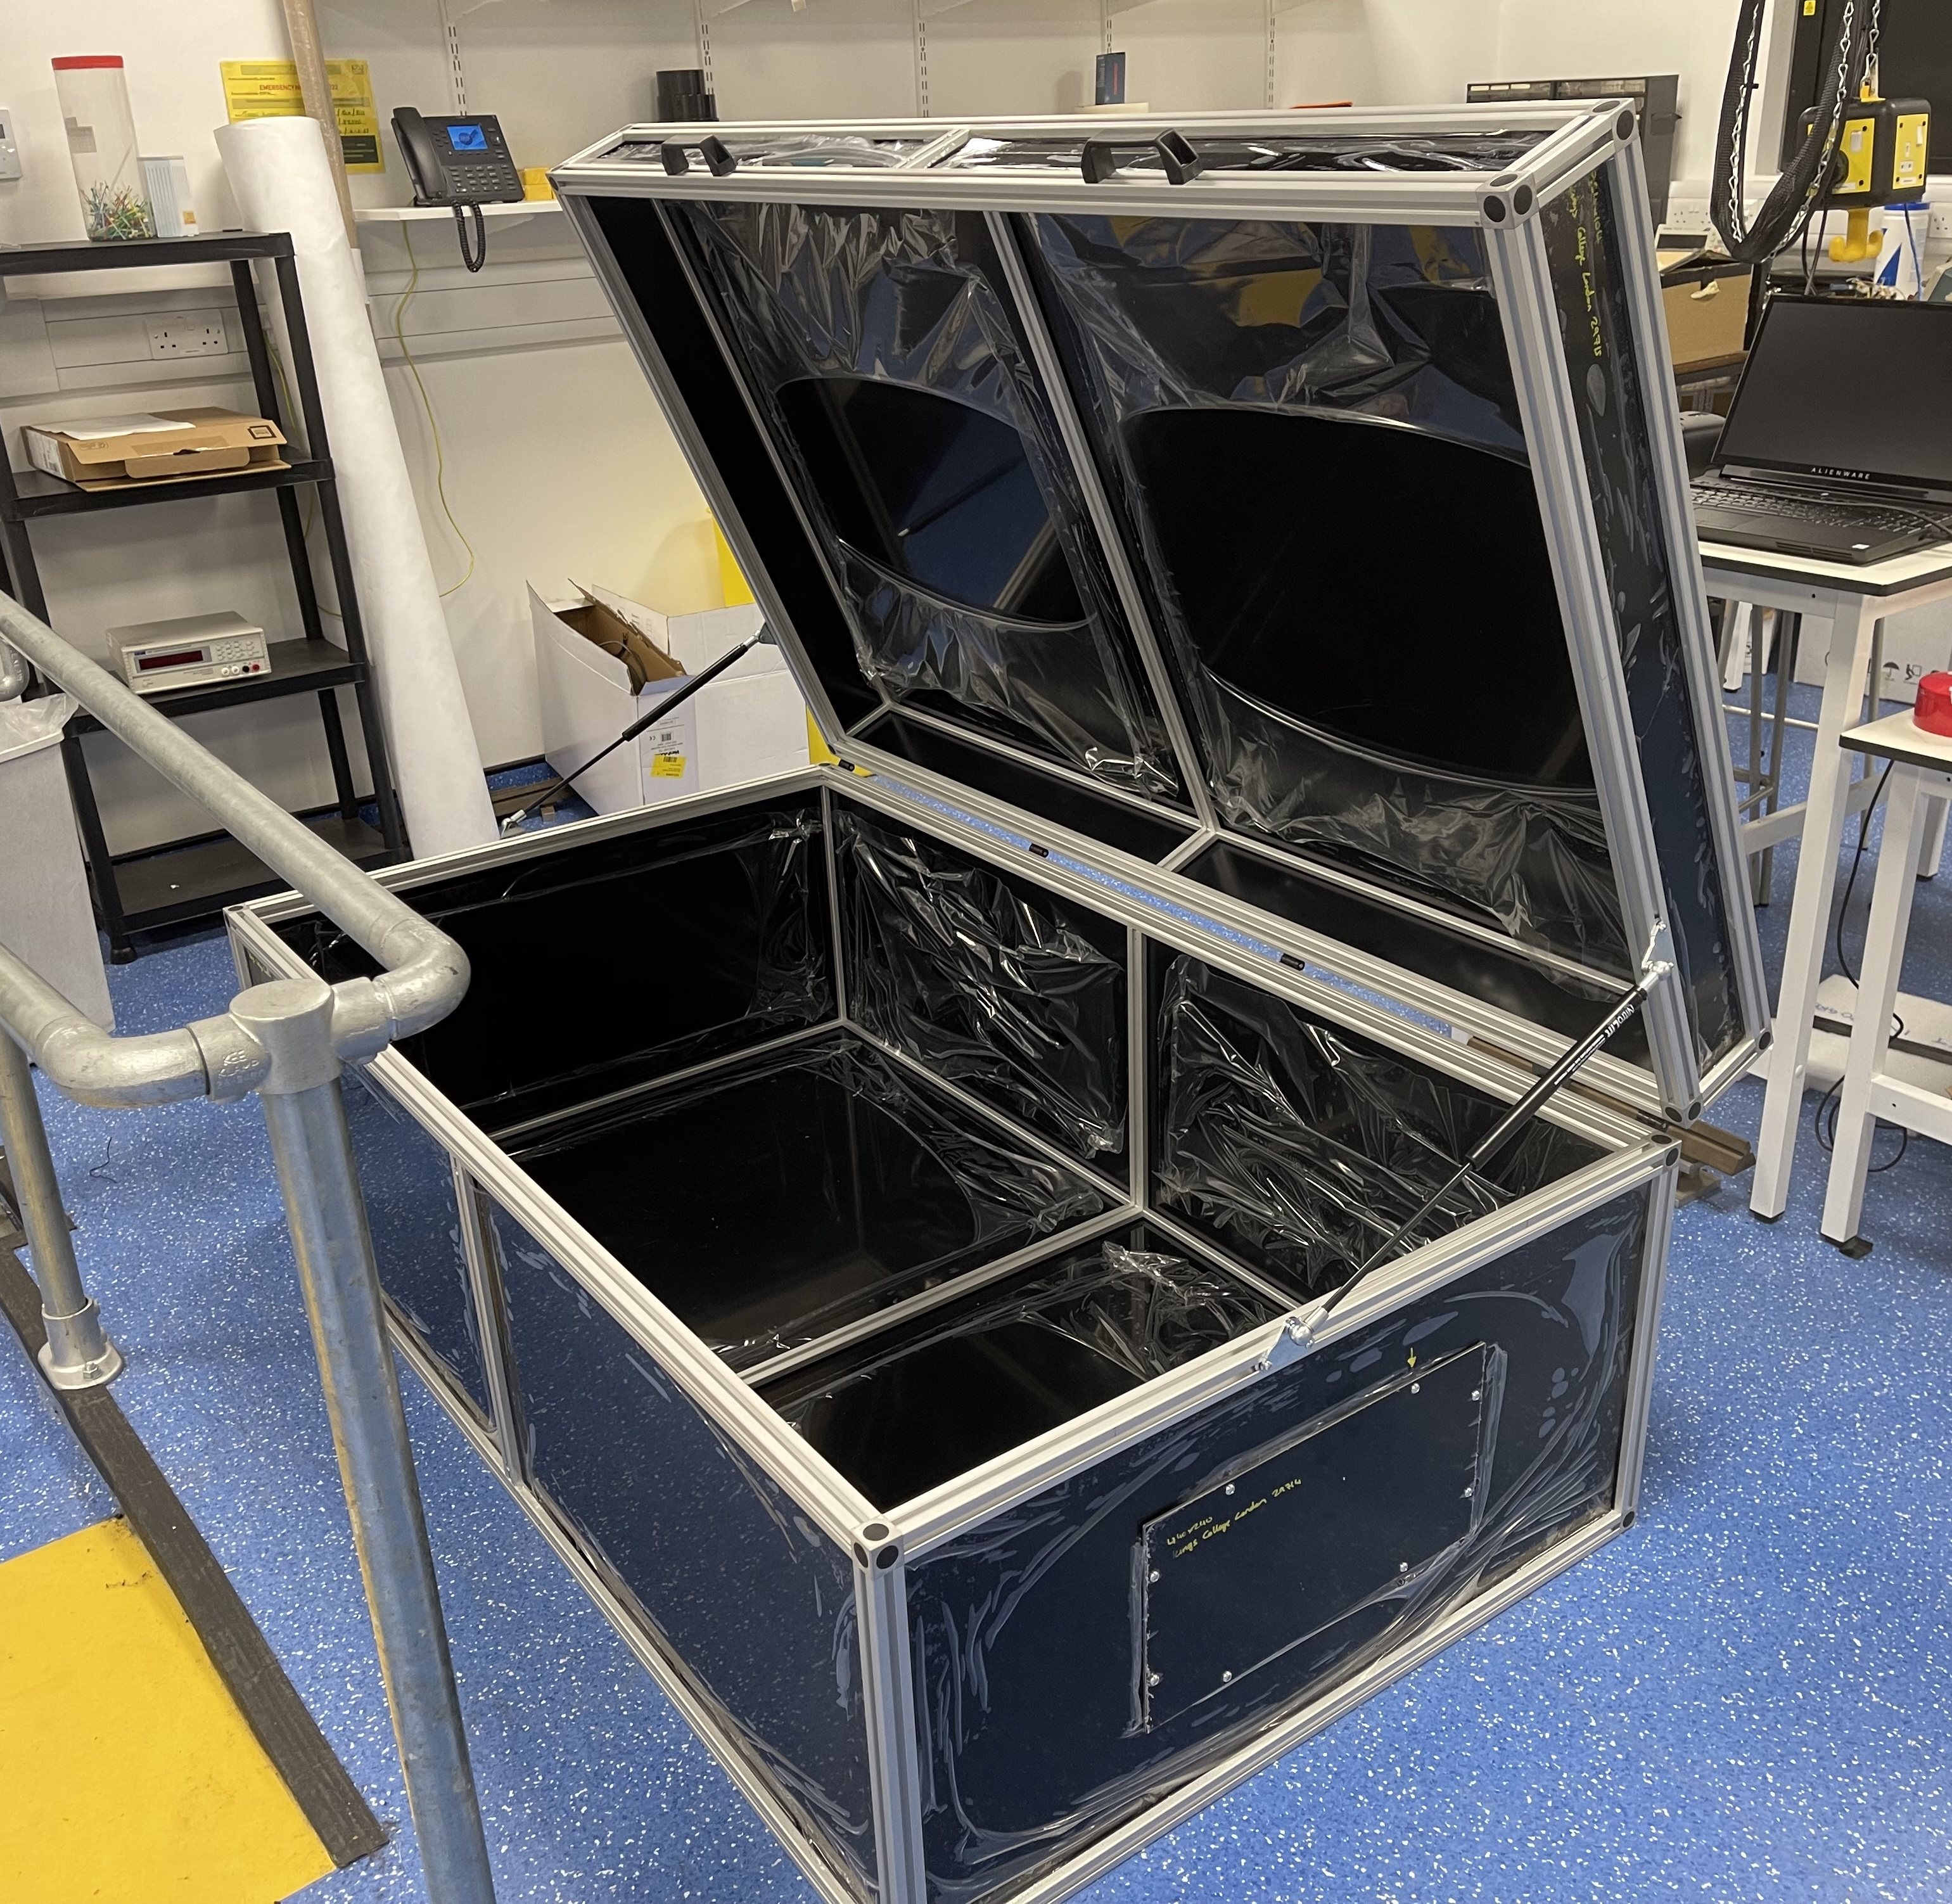
\includegraphics[width=1.\linewidth]{figures/QA_boxes.jpg}
  \caption{Bespoke QA dark box.}
  \label{fig:QA_box}
\end{subfigure}%\
\hfill
\begin{subfigure}{.49\textwidth}
  \centering
  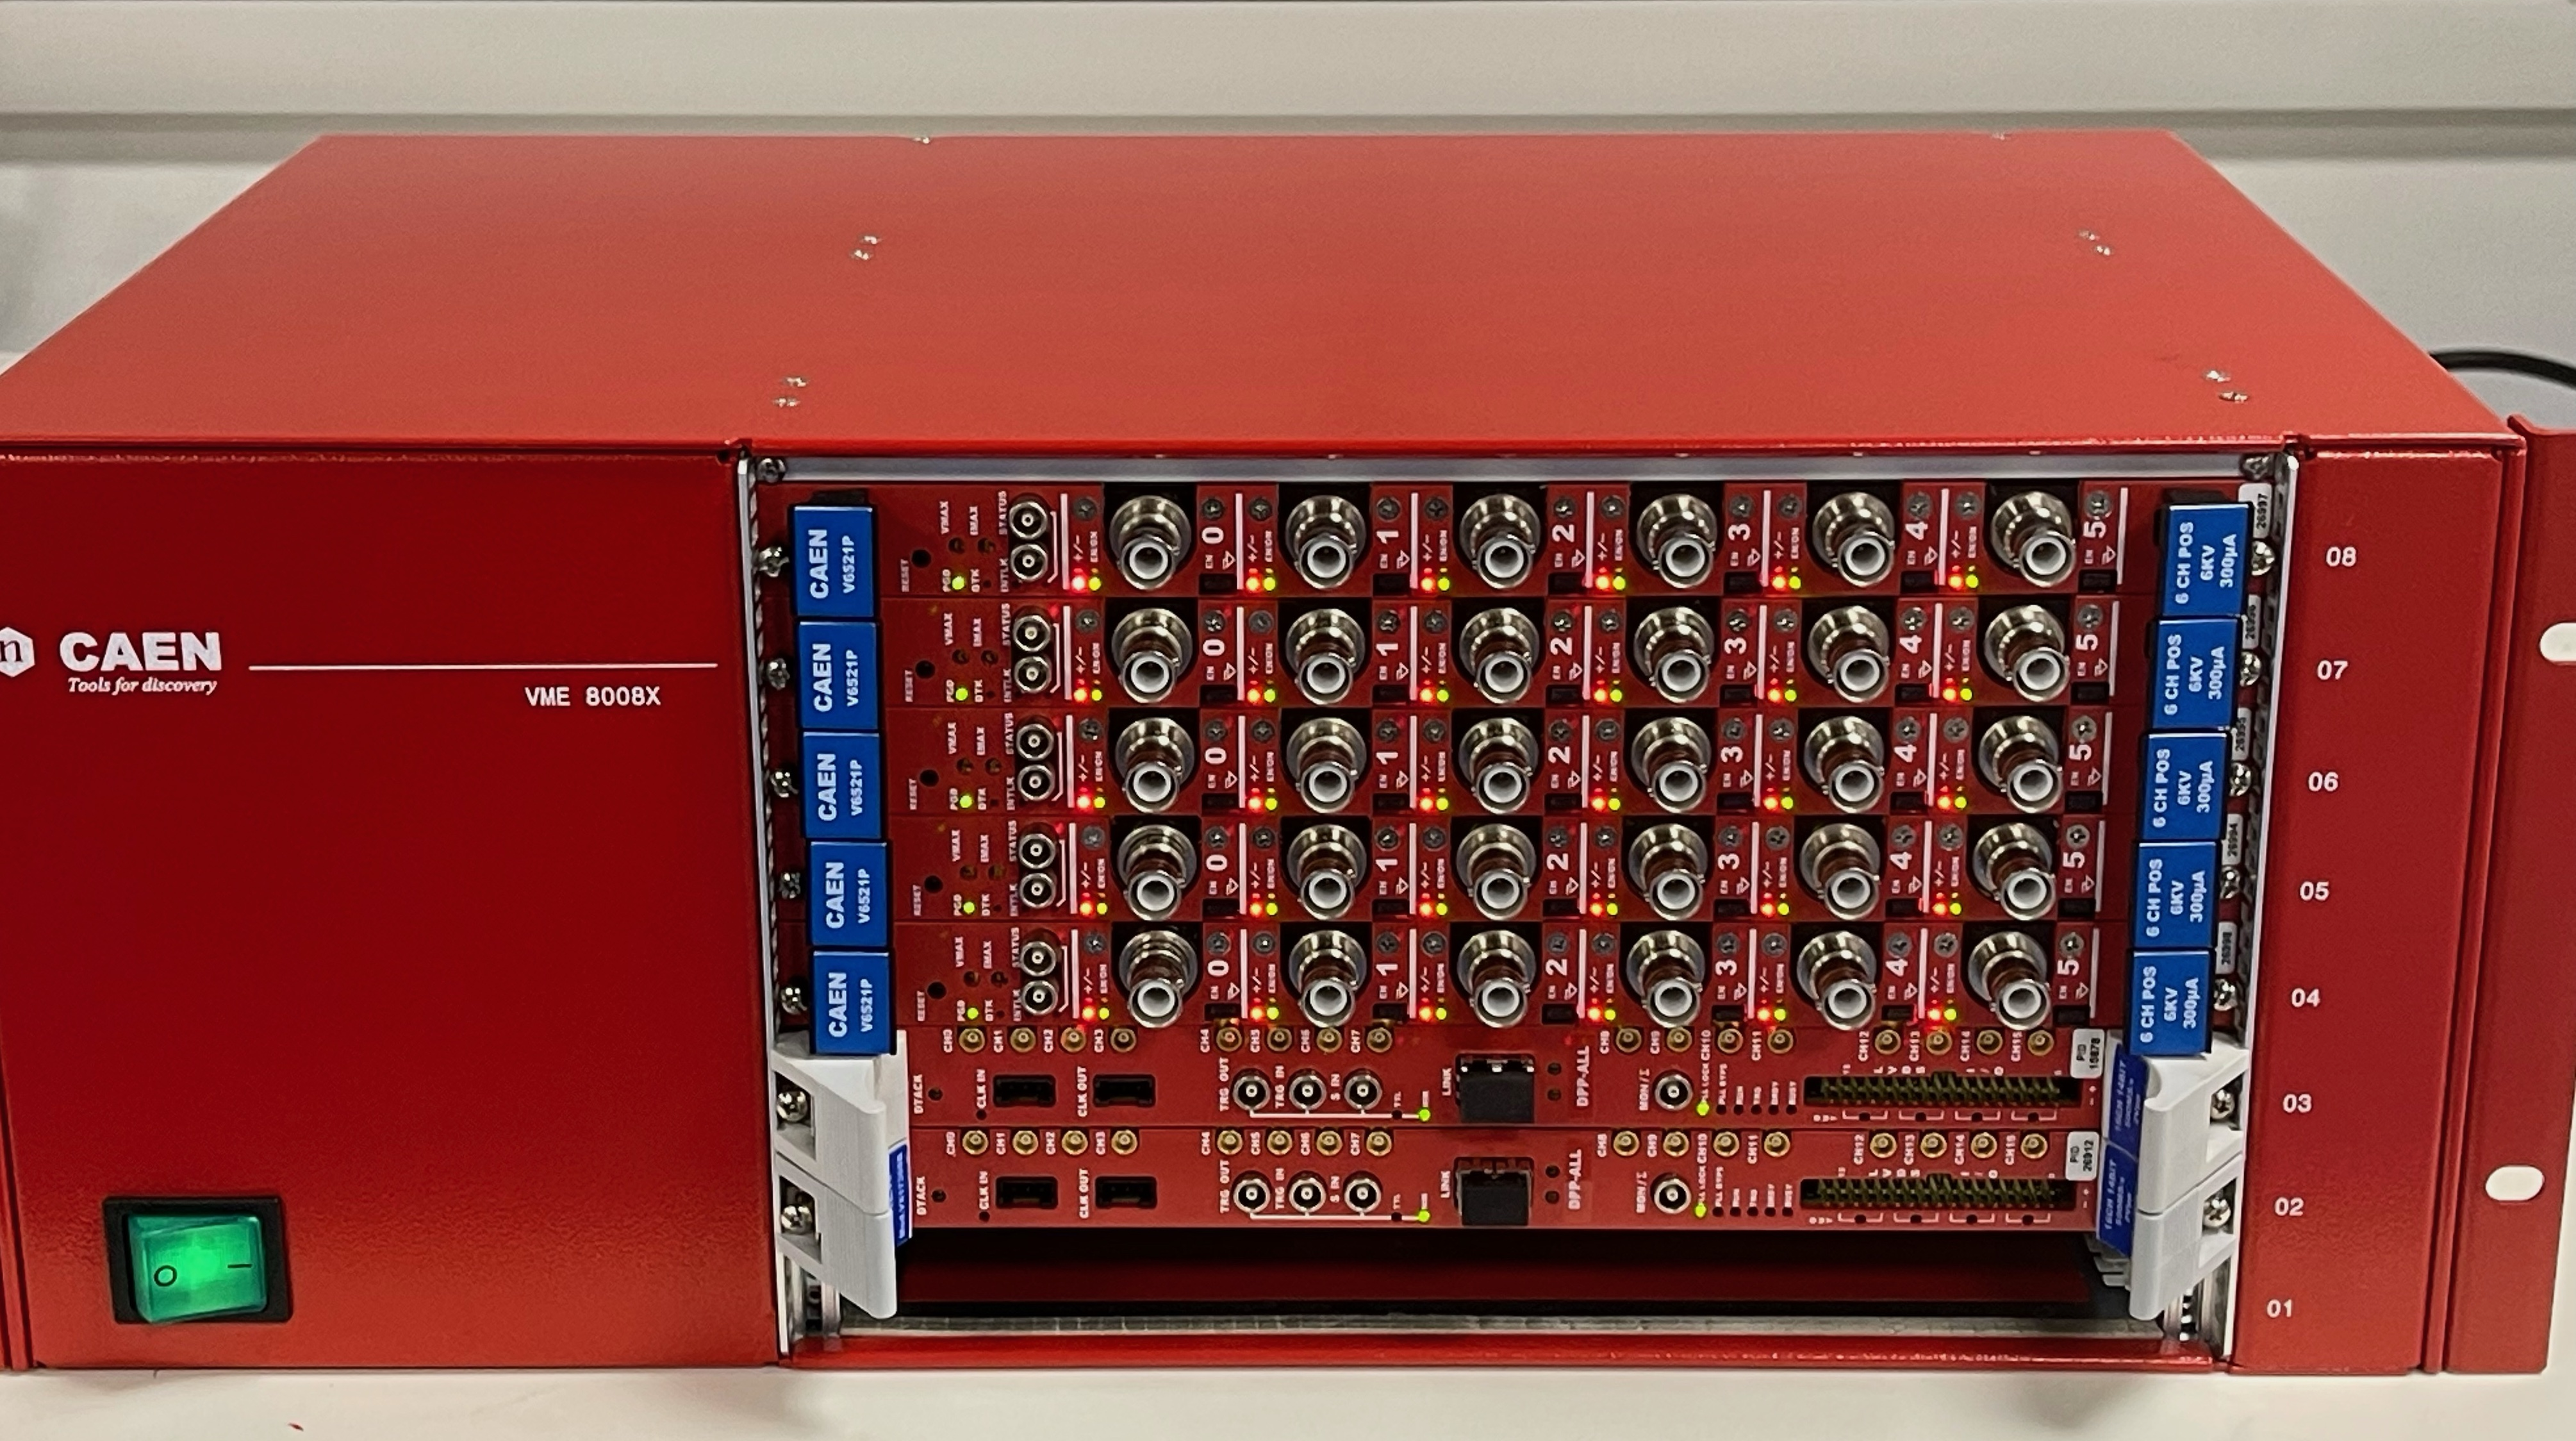
\includegraphics[width=1.\linewidth]{figures/QA_electronics.jpg}
  \caption{VME crate holding the HV and DAQ boards.}
  \label{fig:QA_elec}
\end{subfigure}
\caption{QA setup for batch testing.}
\label{fig:QA_setup}
\end{figure}

\subsubsection{Batch Tests}
The batch tests would be performed in a dark-box with diffuse light sources injected via optical fibres so as to illuminate each PMT with low fixed-intensity, diffuse light. A typical work-flow could involve spending the day installing the PMTs into the dark-box set-up, ramping to nominal high voltage (to allow the PMTs to stabilise in a dark environment for $\ge4$\,hours) and then collecting charge spectra data with the diffuse source at at least three HV settings and dark current measurements overnight. 950\,V is assumed to be the nominal operation voltage and repeated measurements of the gain should be made at this voltage to assess stability over a 12\,hour period. A common reference PMT, that had been characterised in more detail and confirmed to satisfy quantum efficiency (QE) requirements, would remain in the dark box for each set of measurements allowing for the relative QE to be determined. 

\subsubsection{Characterisation Tests}
The characterisation tests would be performed individually in a separate dark-box with a directional light source. This would allow to probe the quantum and collection efficiency either at a small selection of standard LED wavelengths (eg. UV, 420\,nm) or better still, using a monochromator to probe wavelength across the range of interest 300--500\,nm. The measurements would be performed with the PMT in two positions differing by a 90$^\circ$ rotation to test the impact of the Earth's magnetic field. These measurements should be compared against the manufacturers specifications and between the PMTs tested within the supplied batch. Any departure from expectations should be discussed for each batch of PMTs supplied. Further measurements will be performed with the PMT attached to a WLS plate to characterise the efficiency across the whole `PMT unit'. 

A further important property to test is the waterproofing and pressure rating of the PMTs. Since this requires submerging the PMTs in water for measurement, it is not feasible to include in the batch testing process and likely will require a dedicated setup. Such tests should be performed separately on $\ge$1\% of the PMTs to confirm they operate stably under water.

%%%%%%%%%%%%%%%%%%%%%%%%%%%%%%%%%%%%%%%%%%%%%%%%%%%%%%%%%%%%%%%%%%%%%%%%%%%%%%%
%%%%%%%%%%%%%%%%%%%%%%%%%%%%%%%%%%%%%%%%%%%%%%%%%%%%%%%%%%%%%%%%%%%%%%%%%%%%%%%
%%%
%%%                       Quality Assurance procedure
%%%
%%%%%%%%%%%%%%%%%%%%%%%%%%%%%%%%%%%%%%%%%%%%%%%%%%%%%%%%%%%%%%%%%%%%%%%%%%%%%%%
\section{Quality Assurance procedure}\label{secQAProcedure}

General overview of the QA procedures, what measurements we want to do, how much time will each measurement take, how will the day-to-day of the QA shift look like, how many PMTs do we plan to measure,,..?

Should I also discuss the plans for the testing of the QA procedure that will happen in the first half of 2026?

Also describe the integration with the HK database and the shift system, expectations of the shifters and so on.

\subsection{Overview}
\begin{enumerate}
    \item Finish measurements from the previous day/week
    \begin{enumerate}
      \item Finish the dark rate measurement from the previous day/week
      \item Do a preliminary check of the results and finish the QA
      \item Save the measured data and make sure they were correctly loaded into the hk database
      \item Note down the results into the shift logbook
      \item Turn off the PMTs and wait until the application turns green 
    \end{enumerate}
    \item Unload PMTs from the dark boxes
    \begin{enumerate}
      \item Open the dark boxes and disconnect the PMTs from the splitter boards
      \item Unload the PMTs from the dark boxes back into the corresponding boxes (carefully check the labels and the bar codes - separate faulty PMTs)
      \item Move the measured PMTs from previous day/week back into storage room
      \item (once a week) Batch of PMTs arrive into the `GW' storage room in the university of Toyama (batch of 400 PMTs once a month)
      \item Subset of PMTs (84 - 140, corresponding to 3-5 days of PMT QA) is separated and transported into the QA room (30 minutes)
      \item Open the box of PMTs and confirm the PMT labels match with the expectations
    \end{enumerate}
    \item Visual inspection of the PMTs
    \begin{enumerate}
      \item If not already running, start the QA program
      \item One by one perform the visual inspection of the PMTs
    \end{enumerate}
    \item Load the PMTs into the dark boxes
    \begin{enumerate}
      \item Load the PMTs one by one - note the position that the PMT is being loaded to, scan the bar code and connect the PMT to the correct corresponding splitter boards
      \item Close the dark boxes and make sure they are properly light tight
    \end{enumerate}
    \item Test the PMT connection and threshold
    \begin{enumerate}
      \item Measure the pedestal and noise of each PMT vs discriminator threshold
      \item Turn on all the PMTs into their starting voltage (probably done with a single button in the QA programme)
      \item Make sure all the PMTs are turned on a charged and communicate with the programme
      \item Test the PMT signal by recording a single waveform from each PMT
    \end{enumerate}
    \item Leave the PMTs alone for at least an hour (ideally during lunch)
    \item Perform the voltage scan
    \begin{enumerate}
      \item Make sure all PMTs are set to the starting voltage (900 V)
      \item Switch the trigger from the function generator to the LED and check that the LED is on multi-PE setting
      \item Turn off the function generator and turn on the LEDs
      \item Check all PMTs are still connected and perform the voltage scan
      \item Check that all waveforms, charge distributions and gain curves look reasonable (ideally live as the PMTs are being measured)
      \item In the meantime, you can help transport PMTs between storage and QA areas
      \item Once the voltage scan is finished, check the results and save them into the database
    \end{enumerate}
    \item Perform the single PE measurement
    \begin{enumerate}
      \item Change the LED setting to single PE setting
      \item Set all the PMTs to their operational voltage
      \item Do the single PE measurement (should only take about 10 minutes)
      \item Check the results of the single PE measurement
      \item Save the results into the database
      \item Write down the results into the logbook
    \end{enumerate}
    \item Perform the dark rate measurement
    \begin{enumerate}
      \item Turn off the LEDs and turn on the function generator
      \item Turn off the lights and start the dark rate measurement
    \end{enumerate}
    \item Finish the shift
    \begin{enumerate}
      \item Make sure all the results are saved into the database and logbook
      \item Compile a written report and send it to the shift leader/google drive
    \end{enumerate}
\end{enumerate}

\subsection{Shifts}
The QA shifts are expected to take ... hours, with the expectation that the shifters will be able to perform the QA measurements on their own. The shifts will be done in pairs to help with loading and unloading of the PMTS, as well as with transporting the PMTs between the storage and QA areas. The shifters will be expected to perform the measurements, check the results, and save them into the database and logbook.

There should be at least one experienced shift leader near or in Toyama at all times, who will be able to help with the measurements and answer any questions that the shifters might have. The shift leader will also be responsible for checking the results of the measurements and making sure that they are correctly saved into the database and logbook.

\section{Shift software}

\subsection{Data Acquisition software}
The data acquisition software is currently in development, but the idea is to have a simple GUI that will allow the shifters to perform the QA measurements, check the results, and save them into the database and logbook. The software will be able to communicate with the PMTs via CAEN libraries. The control of the function generator and the LEDs will be done manually, but the software will be able to control the PMTs and the data acquisition process.

\subsection{Graphical User Interface}

\subsection{Analysis}

\subsection{Hyper-K database integration}
To load the information from the manufacturer, we will communicate our needs and create a parser script that will automaticall load the information provided in the form of a csv file into the Hyper-K database. This will be decided and designed together with the manufacturer.

%%%%%%%%%%%%%%%%%%%%%%%%%%%%%%%%%%%%%%%%%%%%%%%%%%%%%%%%%%%%%%%%%%%%%%%%%%%%%%%
%%%%%%%%%%%%%%%%%%%%%%%%%%%%%%%%%%%%%%%%%%%%%%%%%%%%%%%%%%%%%%%%%%%%%%%%%%%%%%%
%%%
%%%                         Measurement details
%%%
%%%%%%%%%%%%%%%%%%%%%%%%%%%%%%%%%%%%%%%%%%%%%%%%%%%%%%%%%%%%%%%%%%%%%%%%%%%%%%%
\section{Details of the QA measurements}\label{sec:QAMeasurements}

Go through every measurement that we will be doing, what is the purpose of each measurement, how it will be done, what are the expected results, how to interpret the results, how to report them, how to store them, how to use them in the future.

All the PMTs are placed in the dark box in the same orientation, based on the PMT dynode orientation. The PMTs are connected to the splitter boards, which are connected to the DAQ system. The PMTs are powered by a CAEN power supply, which is controlled by the DAQ software. The function generator is used to trigger the PMTs and the LEDs are used to illuminate the PMTs.

In each dark box, there is one control PMT, which stays in the dark box for the whole duration of the measurements. The dark boxes also contain thermometers and hygrometers to measure the temperature and humidity in the dark box. The temperature and humidity are logged into the database together with the PMT measurements.

\subsection{Visual inspection}
Check for scratches, dents, dark spots, dust, and other imperfections on the PMT glass. Check the condition of the PMT cable and the connector. Check the QR code and make sure it is readable and that it serial number matches between the PMT and the box. If there are any issues, note them down in the logbook and take a picture of the PMT.

The shifter is guided through the visual inspection by the GUI, which will display a checksheet with the items to check. The shifter will be able to mark each item as checked, and if there are any issues, they will be able to add a comment and take a picture of the PMT. The results of the visual inspection will be saved into the Hyper-K database as ``passed'' or ``failed'', with a comment and a picture if there are any issues. The results will also be saved into the logbook.

If there are any serious issues with the PMT, we will send the details to the manufacturer and ask for a replacement. If the issues are minor, we will note them down and continue with the QA process.

Time: 1 min / PMT $\rightarrow$ 30 minutes for one batch of 28 PMTs

\subsection{Voltage scan / Gain measurement}
\note{How many voltage points do we want to take?}
Time: $\sim$6 min / voltage point for all PMTs $\rightarrow$ ~60 minutes for all PMTs including analysis

\subsection{Single Photo Electron measurements}

Time: 10 minutes for all PMTs (maybe more if we want to be very precise)

\subsection{Dark rate measurement}

Time: 12 hours for all PMTs overnight

\subsection{Other measurements}
Relative quantum efficiency, collection efficiency, timing resolution, pressure test, water test, etc.

\section{Conclusion}
Conclusion

\FloatBarrier
\bibliographystyle{unsrturl}
%\bibliography{TestBeamCalibrationTechNoteLiterature}
\end{document}